\documentclass[11pt]{article}
\usepackage{graphicx}
\usepackage{subcaption}
\usepackage{wrapfig}
\title{Ubiquitous Genomics: Hackathon2}

\author{
  Maya Anand\\ mva2112@columbia.edu \and
  Anne Bozack\\ akb2134@cumc.columbia.edu \and
  Cheyenne Parsley\\ cep2141@columbia.edu \and
  Robert Piccone\\ rap2186@columbia.edu \and
  Daniel Speyer\\ dls2192@columbia.edu}
\begin{document}
\maketitle
\section*{Problem 1}
Number of 2D reads classified as failed: 0\\
Number of 2D reads classified as passed: 0\\
\section*{Problem 2}
\begin{wrapfigure}{r}{2.5in}
  \vspace{-20pt}
  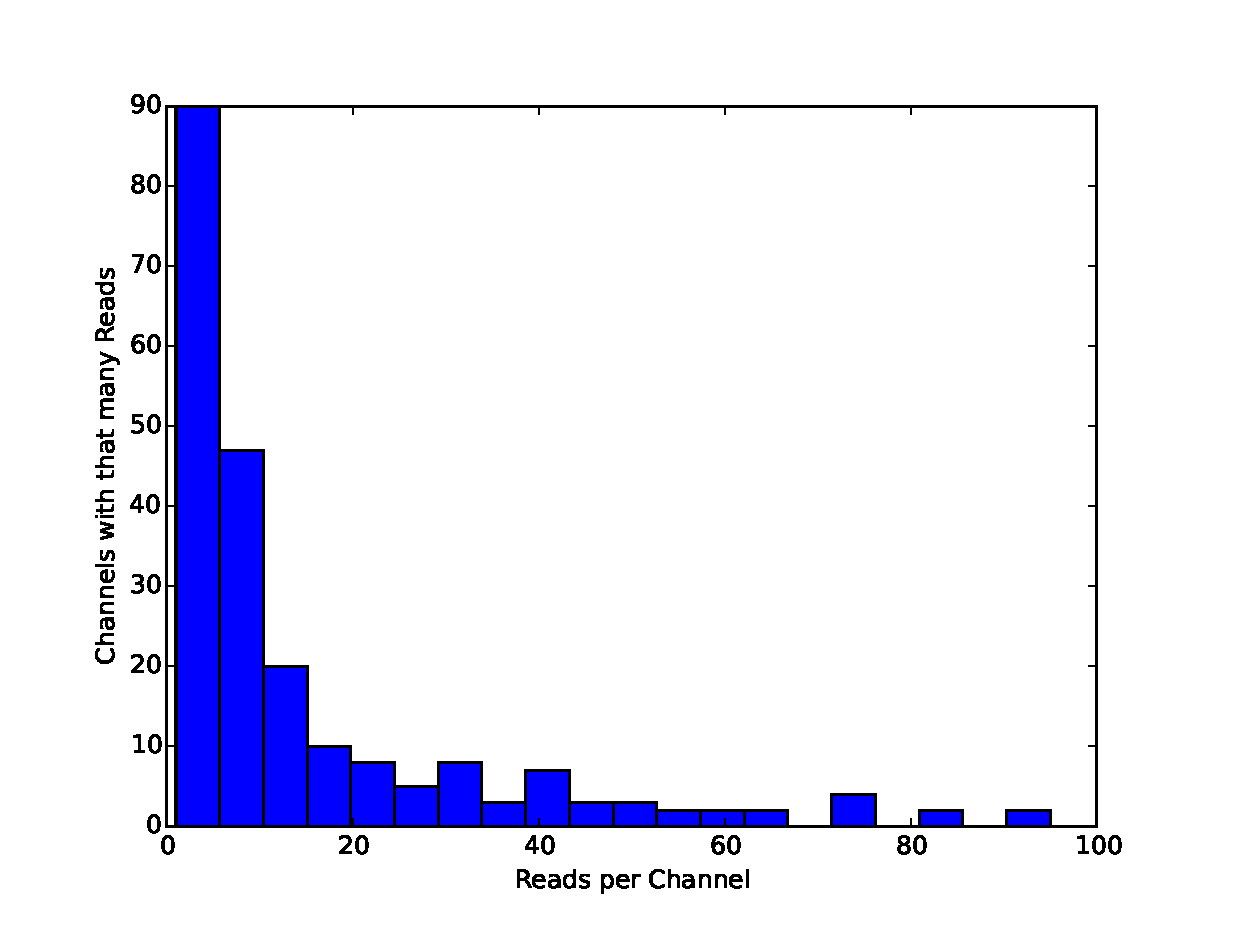
\includegraphics[width=2.5in]{part2hist}
  \vspace{-20pt}
\end{wrapfigure}
0 channels had at least one read, and 0 had at least five.  
This compares with 434 ``active'' channels during initialization, and 651 immediately after loading fuel

\section*{Problem 3}
\subsection*{Failed Reads}

        The following histograms show the length distribution of 2D and 1D reads for fails.

        
        \begin{tabular}{cc}
          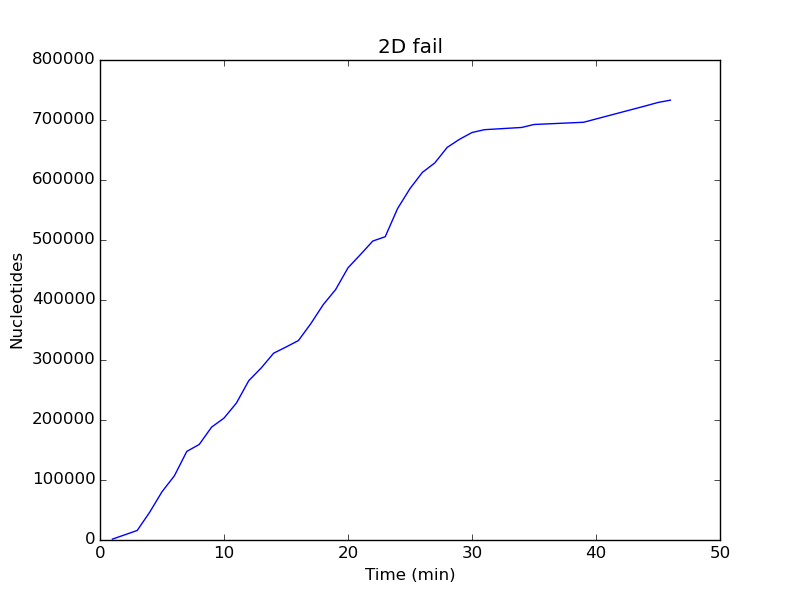
\includegraphics[width=.48\textwidth]{failcum2D}
          &
          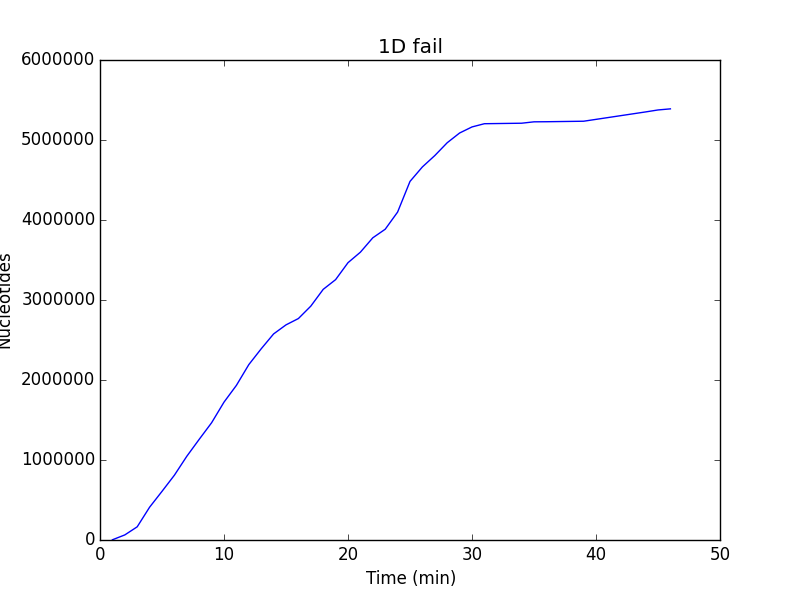
\includegraphics[width=.48\textwidth]{failcum1D}
          \\
          2D Reads
          &
          1D Reads
        \end{tabular}

\subsection*{Passed Reads}

        The following histograms show the length distribution of 2D and 1D reads for passes.

        
        \begin{tabular}{cc}
          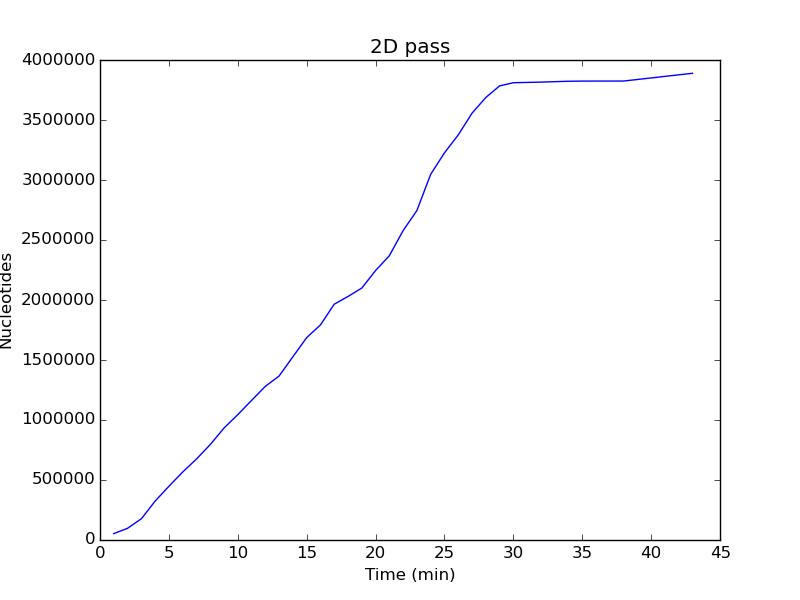
\includegraphics[width=.48\textwidth]{passcum2D}
          &
          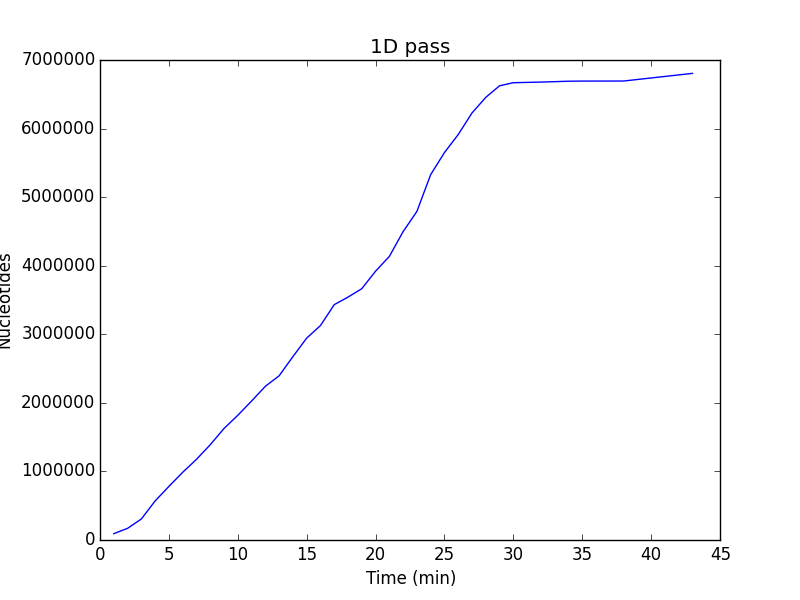
\includegraphics[width=.48\textwidth]{passcum1D}
          \\
          2D Reads
          &
          1D Reads
        \end{tabular}
\section*{Problem 4}
\subsection*{2D reads}

        The following histograms show the length distribution of 2D reads for passes and fails.

        
        \begin{tabular}{cc}
          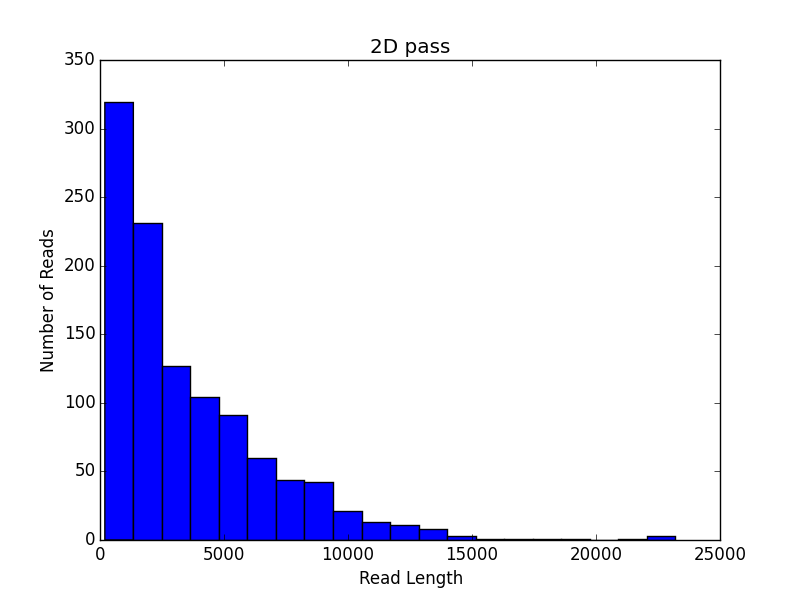
\includegraphics[width=.48\textwidth]{2Dpasses}
          &
          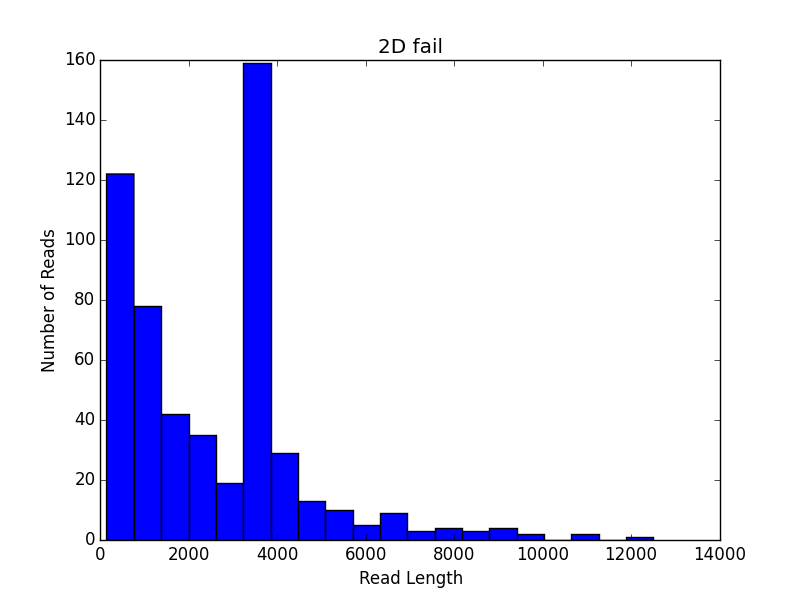
\includegraphics[width=.48\textwidth]{2Dfailures}
          \\
          Passed Reads
          &
          Failed Reads
        \end{tabular}
\section*{Problem 5}

LONGEST PASSED 2D READ\\
From file: .\\
Number of nucleotides: 0\\

LONGEST FAILED 2D READ\\
From file: .\\
Number of nucleotides: 0\\
\section*{Problem 6}
\section*{Problem 7}
\begin{tabular}{r||r|r|r|r|r}
  & A & C & G & T & -\\ \hline
\hline
A & 170885 & 3697 & 4060 & 1611 & 11374\\ 
\hline
C & 2084 & 116750 & 2586 & 2262 & 6074\\ 
\hline
G & 2515 & 2554 & 114255 & 1837 & 6446\\ 
\hline
T & 1741 & 3952 & 3316 & 171694 & 10925\\ 
\hline
- & 10330 & 11696 & 12358 & 9871 & 0\\ 
\end{tabular}
\section*{Problem 8}
\end{document}
